% --- ARCHIVO: Cap2_contexto_sector/contexto_sector.tex ---

\chapter{Contexto del Sector Eléctrico y Transición Energética}
\label{cap:contexto_sector}

\bigskip

\noindent\textbf{Nota preliminar sobre la distribución de fases.}\quad
A lo largo de este capítulo y de los siguientes se hará referencia
recurrente a las cinco fases en que el Comité de Análisis del Consejo
de Seguridad Nacional estructuró cronológicamente el incidente del
28 de abril de 2025: la \textbf{Fase~0} comprende los días previos y la
mañana del 28A, caracterizada por la inestabilidad latente de tensiones;
la \textbf{Fase~1} (12:00--12:30~CEST) corresponde a las oscilaciones
electromecánicas que precedieron al disparo raíz; la \textbf{Fase~2}
(12:32:00--12:33:18~CEST) abarca las primeras pérdidas de generación
asociadas a sobretensión; la \textbf{Fase~3} (12:33:18--12:33:30~CEST)
recoge la cascada de desconexiones que culminó en el cero de tensión;
y la \textbf{Fase~4} (a partir de las 12:33:30~CEST) describe la
reposición progresiva del suministro. La cronología detallada de cada
fase se presenta en los capítulos~\ref{cap:analisis_incidente}
(p.~\pageref{cap:analisis_incidente}) y \ref{cap:reaccion_reposicion}
(p.~\pageref{cap:reaccion_reposicion}).

\bigskip

\section{Evolución de la potencia instalada: análisis histórico del parque generador
y transición hacia un mix dominado por fuentes no síncronas}
\label{sec:evolucion_potencia}

\lettrine[lines=3, lhang=0.1]{A}{} pesar de que la demanda máxima de electricidad en España lleva más de una
década en estancamiento estructural, el parque de generación ha experimentado
una transformación profunda impulsada por los objetivos de descarbonización europeos y el
Plan Nacional Integrado de Energía y Clima (PNIEC). El análisis histórico de los
últimos quince años evidencia un cambio sustancial en la composición del mix:
si en 2010 las fuentes térmicas y nucleares representaban el 65~\% de la
producción, en 2024 las renovables habían invertido esa proporción, alcanzando
el 59~\% del mix total \cite{mitceepr2025}.

\vspace{0.6cm}
\begin{figure}[H]
    \centering
    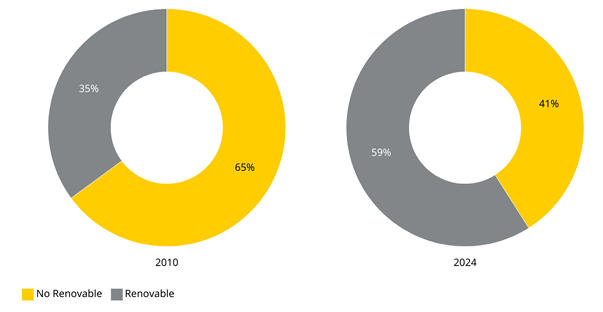
\includegraphics[width=0.7\textwidth]{figuras/mix_comparativo_2010_2024.png}
    \vspace{0.2cm}
    \caption[Evolución macroscópica del mix de generación en España (2010 vs. 2024).]{%
    Evolución macroscópica del mix de generación en España (2010 vs. 2024).
    Fuente: Centro Peter Huber / ESIOS}
    \label{fig:mix_comparativo}
\end{figure}
\vspace{0.6cm}

En el primer cuatrimestre de 2025, el sistema peninsular consolidó este escenario
superando los 100~GW de capacidad renovable instalada. A enero de 2025,
casi el 66~\% de la capacidad total procedía de fuentes descarbonizadas, con energía
eólica y solar fotovoltaica en paridad técnica (24,9~\% cada una). Incluyendo
el autoconsumo distribuido, la cuota fotovoltaica global ascendía a más de
48,1~GW, frente a los 33,1~GW eólicos \cite{ree2025}.

\vspace{0.6cm}
\begin{figure}[H]
    \centering
    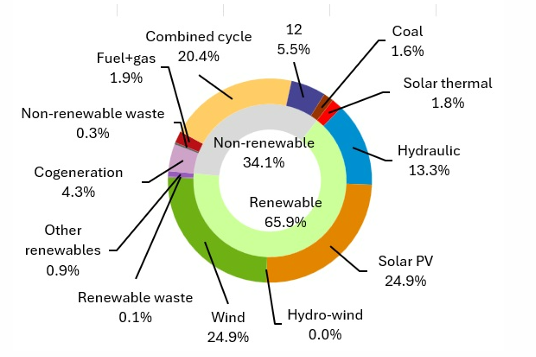
\includegraphics[width=0.8\textwidth]{figuras/capacidad_instalada_2025.png}
    \vspace{0.2cm}
    \caption[Desglose de la capacidad de generación instalada a enero de 2025.]{%
    Desglose de la capacidad de generación instalada en el sistema
    español a 31 de enero de 2025. Fuente: NREL / Red Eléctrica}
    \label{fig:donut_capacidad}
\end{figure}
\vspace{0.6cm}

Como contrapartida directa a la situación presentada, la generación síncrona
convencional ha sido progresivamente desplazada en el orden de mérito. El parque
de carbón ha quedado relegado a un papel residual (1,6~\% de la capacidad
instalada), el nuclear (5,5~\%) afronta un calendario de cierre progresivo, y
los más de 26~GW de ciclo combinado de gas (20,4~\%) operan con factores de
utilización inferiores al 15~\% anuales \cite{gobierno2025}.

Desde la perspectiva de la ingeniería de sistemas de potencia, esta alteración
acelerada de la matriz electromecánica plantea retos operativos relevantes. La
estabilidad histórica de las redes ha venido descansando en los generadores
síncronos ---centrales térmicas, nucleares e hidráulicas--- cuyas masas rotativas
aportan energía cinética ($E_k$) inmediata, inercia física y elevadas corrientes de
cortocircuito ante cualquier perturbación \cite{futured2024}.

La práctica totalidad de las nuevas instalaciones solares y eólicas se conectan, en
cambio, mediante inversores (de ahí su denominación \textit{Inverter-Based
Resources}, IBR). Estos convertidores operan en modo estándar como
``seguidores de red'' (\textit{grid-following}): sincronizan su exportación con la tensión
y frecuencia externas a través de algoritmos tipo PLL (\textit{Phase-Locked Loop}) y, al carecer
de masas rotativas, no aportan inercia síncrona ni responden intrínsecamente a
las fluctuaciones de la red \cite{nrel2025}.

El resultado de esta sustitución es que el sistema ibérico opera de forma
rutinaria bajo un régimen característico de las redes con baja capacidad de
cortocircuito y elevada impedancia. La desconexión progresiva de los
turboalternadores reduce la inercia síncrona total y amplifica la Velocidad de
Cambio de Frecuencia (\textit{Rate of Change of Frequency} RoCoF, $df/dt$) ante
desequilibrios de potencia activa. Más allá de la dinámica de frecuencia, la merma
de máquinas síncronas reduce las fuentes y sumideros dinámicos de potencia
reactiva ($Q$) disponibles en la red, lo que afecta a la capacidad del sistema
para mantener la estabilidad de tensión ($V$) ante variaciones rápidas en los
flujos de la red de transporte de 400~kV \cite{icai2025}.

\clearpage

\section{Intensidad de emisiones del sistema ibérico: el factor de emisiones como motor
de la transformación de la red}
\label{sec:intensidad_emisiones}

La transformación topológica y operativa del sistema eléctrico ibérico durante
las dos últimas décadas se enmarca en el contexto regulatorio común a toda la
Unión Europea: el imperativo legal y medioambiental de descarbonizar la
economía. La reducción de la intensidad de emisiones de Gases de Efecto
Invernadero (GEI) ha sido el motor de la planificación energética nacional,
impulsando la sustitución de tecnologías convencionales vinculadas a fuentes
fósiles por fuentes renovables. Conviene subrayar, no obstante, que estos
objetivos son compartidos por la totalidad de los Estados miembros de
ENTSO-E; los efectos sobre la dinámica del sistema, que este capítulo
describe, son por tanto comunes al área síncrona europea, sin que de ello
pueda inferirse una relación causal directa con el incidente del 28 de abril
de 2025, cuyas causas específicas se analizan en los capítulos posteriores.

A comienzos de siglo, el sistema peninsular presentaba una alta intensidad de
carbono: aproximadamente el 56~\% de la electricidad producida procedía de
centrales térmicas de combustibles fósiles, predominantemente carbón, con
presencia significativa de fuelóleo y de un parque de ciclo combinado de gas
natural en rápida expansión a partir de 2002. Las emisiones absolutas del
sector eléctrico continuaron creciendo hasta alcanzar su máximo histórico
en 2007, próximo a los 110~MtCO$_2$-eq anuales. A partir de esa fecha, los
compromisos derivados del Protocolo de Kioto y, posteriormente, del Acuerdo
de París (COP21) impulsaron un cambio de paradigma regulatorio. Este esfuerzo
se concretó en el Plan Nacional Integrado de Energía y Clima (PNIEC), cuya
actualización fijó el objetivo de que, en 2030, el 81~\% de la generación
eléctrica nacional procediera de fuentes libres de emisiones. En paralelo, el
aumento progresivo del coste de los derechos de emisión de $\text{CO}_2$ en
el mercado europeo (\textit{Emission Trading Scheme}) afectó muy
negativamente a la competitividad de las centrales térmicas de carbón ---como
consecuencia de su eficiencia moderada y de la composición del combustible---,
precipitando su cierre masivo a partir de 2010 \cite{gobierno2025}.

\vspace{0.6cm}
\begin{figure}[H]
    \centering
    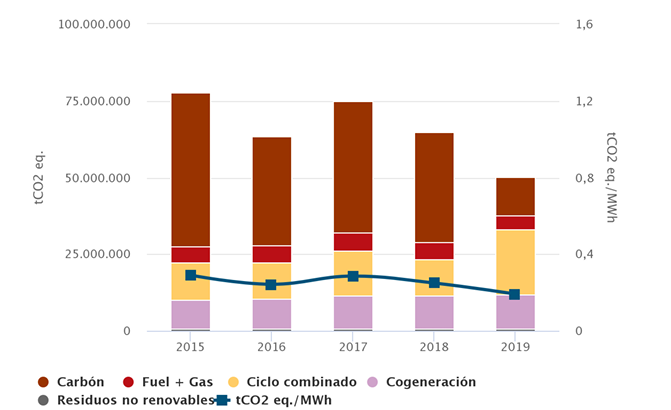
\includegraphics[width=0.85\textwidth]{figuras/esios_emisiones_historico.png}
    \vspace{0.2cm}
    \caption[Evolución histórica de las emisiones de GEI y del factor de emisión en España.]{%
    Evolución histórica de las emisiones absolutas de GEI y del factor de
    emisión específico en el sistema eléctrico español desde 1990. Se
    observa el crecimiento sostenido hasta el máximo de 2007 y el descenso
    posterior, que ha llevado las emisiones actuales a niveles próximos
    a los registrados a comienzos de los años noventa.
    Fuente: e·sios / Red Eléctrica}
    \label{fig:esios_emisiones}
\end{figure}
\vspace{0.6cm}
\clearpage
El éxito ambiental de esta política se refleja en la evolución del factor de
emisión específico del sistema, expresado en toneladas de $\text{CO}_2$
equivalente por megavatio-hora ($\text{tCO}_2\text{eq/MWh}$) o,
equivalentemente, en gramos de $\text{CO}_2$ por kilovatio-hora
($\text{g CO}_2/\text{kWh}$). En 2015, el sistema emitía cerca de
80~MtCO$_2$-eq con un factor de 0,29~tCO$_2$-eq/MWh
($\approx 290~\text{g CO}_2/\text{kWh}$); en 2019, ese factor ya había
descendido a 0,19~tCO$_2$-eq/MWh ($\approx 190~\text{g CO}_2/\text{kWh}$).

La tendencia indicada se ha acelerado en los últimos años, previos al cero de
tensión. Al cierre de 2024, coincidiendo con el máximo histórico de generación
renovable (56,8~\%), las emisiones del sector eléctrico se redujeron hasta
los 27,0~millones de toneladas de $\text{CO}_2$ equivalente, un descenso del
16,8~\% respecto a 2023 y del 75,7~\% frente al pico de 2007 \cite{ree2025}.

\vspace{0.6cm}
\begin{figure}[H]
    \centering
    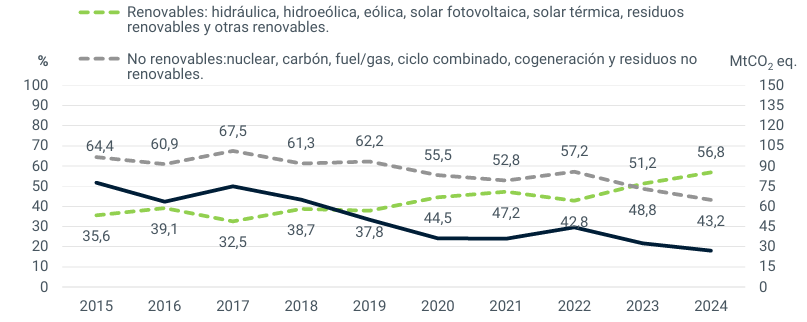
\includegraphics[width=0.85\textwidth]{figuras/ree_emisiones_renovables_2024.png}
    \vspace{0.2cm}
    \caption[Evolución comparativa de la cuota renovable frente a las emisiones absolutas (2015-2024).]{%
    Evolución comparativa de la cuota de generación renovable frente a las
    emisiones absolutas del sistema eléctrico español
    (MtCO$_{2,\text{eq}}$) entre 2015 y 2024.
    Fuente: Red Eléctrica}
    \label{fig:ree_emisiones_2024}
\end{figure}
\vspace{0.6cm}

Desde la perspectiva de la ingeniería de sistemas de potencia, esta reducción
de la intensidad de emisiones constituye un éxito medioambiental indiscutible.
Su contrapartida operativa es que la sustitución de centrales térmicas por
fuentes renovables conectadas a través de inversores conlleva la retirada
progresiva de las masas síncronas que aportaban inercia, potencia de
cortocircuito y control dinámico de tensión. La transición acelerada hacia un
modelo de bajas emisiones ha llevado al sistema ibérico a operar habitualmente
en regímenes de baja inercia y reducida robustez nodal, condiciones cuya
relación con la inestabilidad de tensión observada el 28 de abril de 2025 se
analiza ---confrontando las posiciones divergentes de los distintos agentes
institucionales--- en el capítulo~\ref{cap:analisis_informes}
(p.~\pageref{cap:analisis_informes}).

\section{Estado operativo en los días previos (abril de 2025): balance de potencias y recurso hídrico y eólico disponible}
\label{sec:estado_operativo_previo}

En los días previos al apagón, en particular durante la mañana del 28 de abril
de 2025, el sistema eléctrico peninsular operó bajo unas condiciones que la
literatura técnica ha denominado la ``Paradoja de la abundancia''. Las
temperaturas primaverales inusualmente suaves (en torno a 25~\textcelsius)
y el calendario festivo en diversas regiones deprimieron la curva de demanda: a las
12:30~CEST, escasos minutos antes del colapso, la demanda instantánea se
situaba en 25.184~MW, el 56~\% de la demanda punta histórica del sistema.

Este escenario de demanda valle coincidió con una excepcional disponibilidad de
recurso renovable, de modo que la generación no síncrona cubría el 82~\% del
mix instantáneo. El balance estuvo dominado por la energía solar fotovoltaica,
con aproximadamente 18.000~MW (53~\% del total), complementada
por la eólica con cerca de 3.500~MW (11~\%).

Para equilibrar este volumen de potencia activa ($P$), dada la baja demanda
interna, el sistema recurrió simultáneamente a dos sumideros principales. Por
un lado, al bombeo hidráulico para almacenar parte del excedente de producción
solar: a las 12:30~CEST, las centrales de bombeo consumían cerca de
3.000~MW. Por otro, a la exportación neta hacia los tres sistemas vecinos
---Francia, Portugal y Marruecos---, que actuaron de hecho como sumideros
externos de la sobreproducción peninsular. Esta configuración resultaría
relevante en la fase de colapso: tras el inicio de la cascada, REE se vio
obligada a comunicar a los operadores francés (RTE) y portugués (REN) la
necesidad de reducir las exportaciones programadas, dado que el sistema
ibérico había pasado en pocos segundos de excedentario a deficitario en
potencia activa. Como contrapartida directa al despacho de generación
descrito, la generación síncrona convencional quedó desplazada a mínimos
históricos: el parque nuclear aportaba un 10~\% (3,4~GW) y los ciclos
combinados de gas (CCGT) se reducían a un exiguo 3~\% (aproximadamente
1.600~MW) \cite{ree2025}.

\begin{figure}[H]
    \centering
    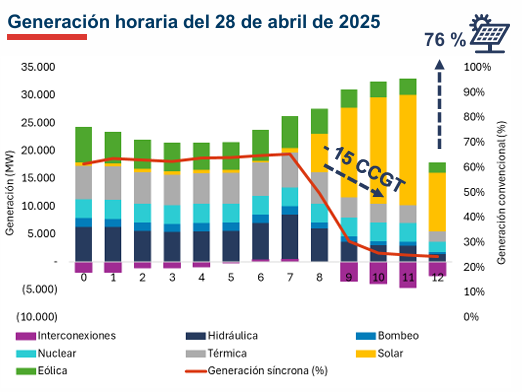
\includegraphics[width=0.75\textwidth]{figuras/ree_generation_mix_28april.png}
    \vspace{0.2cm}
    \caption[Perfil de generación del sistema peninsular el 28 de abril de 2025.]{%
    Perfil de generación del sistema peninsular el 28 de abril de 2025.
    Fuente: NREL / Red Eléctrica}
    \label{fig:perfil_generacion_28abril}
\end{figure}

La figura~\ref{fig:perfil_generacion_28abril} ilustra cómo el valle de
demanda coincidió con un pico extremo de producción fotovoltaica, lo que
desplazó la generación síncrona a niveles mínimos y obligó al uso intensivo
de los sumideros de potencia activa mencionados (bombeo hidráulico y
exportación a los tres sistemas vecinos).

Esta reducción de masas rotatorias se tradujo en valores de inercia notablemente
bajos en algunas zonas del sistema. Los registros periciales indican que la
inercia síncrona cayó a 1,3~s en el área Sur y 1,84~s en el área Centro, por
debajo del umbral de 2~s recomendado por la \textit{Red Europea de Gestores de Redes
de Transporte de Electricidad (ENTSO-E)}\textsuperscript{\ref{anexo:entsoe}}. La operación prolongada en
estas condiciones ya había producido señales de estrés dinámico los días 16,
22 y 24 de abril, en los que se registraron episodios de inestabilidad de
tensión en la red de transporte \cite{icai2025}.

\begin{figure}[H]
    \centering
    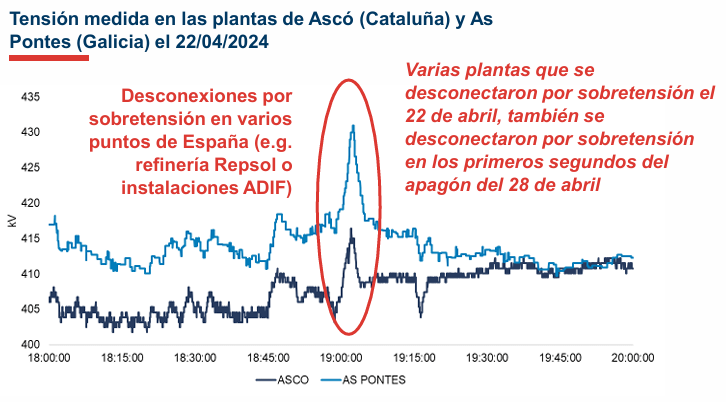
\includegraphics[width=0.75\textwidth]{figuras/precursor_overvoltage_22april.png}
    \vspace{0.2cm}
    \caption[Oscilaciones de tensión registradas en Núñez de Balboa el 22 de abril de 2025.]{%
    Oscilaciones de tensión registradas en la subestación de Núñez de Balboa
    (tensión nominal 400~kV) durante el episodio precursor del 22 de abril
    de 2025. Fuente: Informe preliminar IIT-ICAI / Compass Lexecon}
    \label{fig:oscilaciones_precursoras}
\end{figure}

La figura~\ref{fig:oscilaciones_precursoras} recoge las oscilaciones de
tensión registradas en la subestación de Núñez de Balboa (red de transporte
de 400~kV) durante el episodio del 22 de abril, considerado por el informe
ICAI como representativo de los precursores que se observaron en los días
previos. Este tipo de transitorios es interpretado por dicho informe como
indicio del estrechamiento de los márgenes de control de potencia reactiva
en la red de transporte.



El antecedente más severo ocurrió el martes 22 de abril, en torno a las
19:00~horas. Una confluencia de factores operativos ---gradientes pronunciados
de bajada de generación solar y cambios bruscos en los flujos de
interconexión--- desencadenó un pico de sobretensión superior a 430~kV.
Este transitorio activó las protecciones de red y provocó la desconexión de
múltiples plantas, principalmente fotovoltaicas y eólicas conectadas mediante
inversores; significativamente, varias de las instalaciones que dispararon
por sobretensión en los primeros segundos del apagón del 28 de abril ya
habían sufrido disparos idénticos durante este evento previo \cite{icai2025}.

Analizados en conjunto, estos episodios sugieren que el sistema peninsular
operaba con sus márgenes de control dinámico de tensión estructuralmente
estrechos. La elevada penetración de recursos basados en inversores (IBR),
combinada con la desconexión de los grupos síncronos convencionales,
disminuyó la capacidad de la red para gestionar potencia reactiva de forma
dinámica, configurando las condiciones operativas en las que se desencadenó
el incidente del 28 de abril de 2025.

\section{Capacidad de las interconexiones: límites de intercambio técnico y
comercial con Francia (RTE) y Marruecos}
\label{sec:interconexiones}

\subsection{La península ibérica como ``isla energética''}

Para comprender la dinámica del sistema eléctrico peninsular es necesario
definir su posición estructural dentro del área síncrona de Europa
Continental (ENTSO-E). Geográfica y eléctricamente, la península ibérica
opera bajo la condición de ``isla energética'': sus interconexiones
transfronterizas a través de los Pirineos son débiles en relación con el
tamaño del sistema. La capacidad de intercambio entre España y Francia se
sitúa históricamente entre el 3~\% y el 5~\% de la capacidad de generación
instalada ---o un 7,9~\% medido frente a la demanda punta---, valores
inferiores al objetivo vinculante del 15~\% fijado por la Unión Europea
para 2030 \cite{mitceepr2025}. Esta limitación topológica condiciona la
seguridad del suministro. Al situarse en el extremo periférico de la red
síncrona, el sistema ibérico experimenta un denominado ``efecto látigo'':
las perturbaciones originadas en el centro de inercia europeo se amplifican
al propagarse hacia la península. Además, ante una pérdida masiva de
generación, el cuello de botella de las interconexiones limita físicamente
la inercia y el soporte dinámico que España puede importar de los grandes
alternadores centroeuropeos \cite{entsoe2025}.

\subsection{Límites de intercambio: comercial (NTC) frente a físico (técnico)}

Es indispensable distinguir entre los límites comerciales y los flujos físicos reales.
Desde la perspectiva del mercado, los intercambios se rigen por la Capacidad
Neta de Transferencia (\textit{Net Transfer Capacity}, NTC), un valor pactado
\textit{ex ante} entre Red Eléctrica de España (REE, operador técnico del sistema español) y Réseau de Transport d'Électricité (RTE, operador técnico del sistema francés). Sin embargo, en regímenes transitorios rápidos,
los flujos físicos de potencia activa ($P$) y reactiva ($Q$) obedecen las Leyes de
Kirchhoff y los criterios de estabilidad angular, con independencia de los
programas de mercado \cite{entsoe2025}. Forzar un flujo físico por encima del límite de estabilidad angular ---típicamente
90\textdegree\ de diferencia entre ambos extremos--- no incrementa la potencia
transferida, sino que provoca una divergencia de polos y la consiguiente pérdida
de sincronismo, mecanismo que se materializó el 28 de abril a las 12:33:21~CEST
\cite{ree2025}.

\begin{figure}[H]
    \centering
    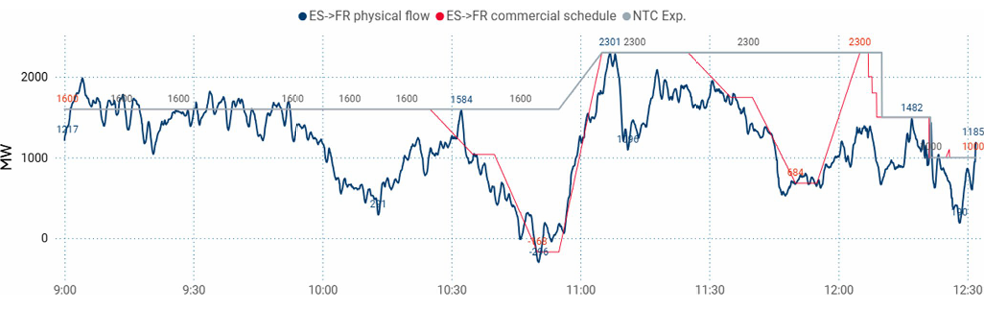
\includegraphics[width=0.85\textwidth]{figuras/entsoe_flow_deviation.png}
    \caption[Desviación entre programa comercial (NTC) y flujo físico en la frontera ES-FR.]{%
    Desviación entre el programa de intercambio comercial (NTC) y el flujo
    de potencia físico real en la frontera España-Francia durante la mañana
    del 28 de abril.
    Fuente: Informe Factual ENTSO-E}
    \label{fig:entsoe_flow}
\end{figure}

\subsection{Frontera norte (Francia): el doble papel de los enlaces en corriente alterna (AC) y continua (HVDC)}

La interconexión con Francia combina líneas aéreas de corriente alterna (\textit{Alternate Current}, AC) con
el enlace subterráneo de corriente continua de alta tensión (\textit{High Voltage Direct Current Voltage Source Converter}, HVDC VSC) entre
Santa Llogaia y Baixas, denominado INELFE-1, con una capacidad nominal de
2.000~MW \cite{ree2025}.

El enlace HVDC INELFE-1 admite varios modos de operación. En modo
\textbf{PMODE1} (potencia constante) el convertidor mantiene fija una
consigna de potencia activa pactada \textit{ex ante} con los operadores de
ambos extremos, sin reaccionar a las desviaciones de frecuencia o tensión
del sistema. En modo \textbf{PMODE2} se introduce un bucle de control que
modula la potencia transferida en función del desvío de frecuencia,
permitiendo al enlace contribuir al amortiguamiento de transitorios
electromecánicos. En modo \textbf{PMODE3} (emulación AC) el enlace
adapta la potencia transferida a la diferencia angular entre las tensiones
de ambos extremos, comportándose funcionalmente como una línea de
corriente alterna y permitiendo que las oscilaciones interárea se
distribuyan a través del enlace. La elección entre uno u otro modo se
adopta de forma coordinada entre REE y RTE en función del estado operativo
del sistema y de los protocolos bilaterales acordados.

Durante los prolegómenos del apagón, el enlace HVDC operaba inicialmente en
modo PMODE3, lo que le permitía reaccionar a la diferencia angular de las
tensiones en ambos extremos. Sin embargo, a las 12:08~CEST, con el fin de
amortiguar las oscilaciones de 0,6~Hz detectadas en el sistema, el modo de
control se modificó a PMODE1, fijando una exportación de 1.000~MW hacia
Francia \cite{icai2025}.

Esta decisión tuvo consecuencias relevantes en la fase posterior del
incidente. En el momento del colapso, las líneas AC transpirenaicas
intentaron actuar como vía de importación de emergencia, llegando a
solicitar hasta 4.609~MW desde Francia para contener la cascada de
desconexiones internas. Simultáneamente, el enlace HVDC ---fijado en
PMODE1 desde las 12:08~CEST--- continuó extrayendo 1.000~MW del sistema
ibérico hacia Francia, al carecer de un bucle de control de frecuencia
activo que pudiese invertir el sentido del flujo o reducir la consigna ante
la caída de frecuencia peninsular. El resultado neto fue que el soporte
efectivo desde el sistema francés se vio reducido respecto al máximo
teórico disponible si el enlace hubiese permanecido en un modo dinámico.
Esta cuestión ---si la decisión de mantener el HVDC en PMODE1 hasta el
último instante limitó la capacidad de defensa de la frontera pirenaica---
constituye uno de los puntos analizados en detalle en el
capítulo~\ref{cap:analisis_informes}
(p.~\pageref{cap:analisis_informes}). A las 12:33:21~CEST, las líneas AC
abrieron por pérdida de sincronismo, aislando totalmente la península del
sistema síncrono continental \cite{entsoe2025}.

\begin{figure}[H]
    \centering
    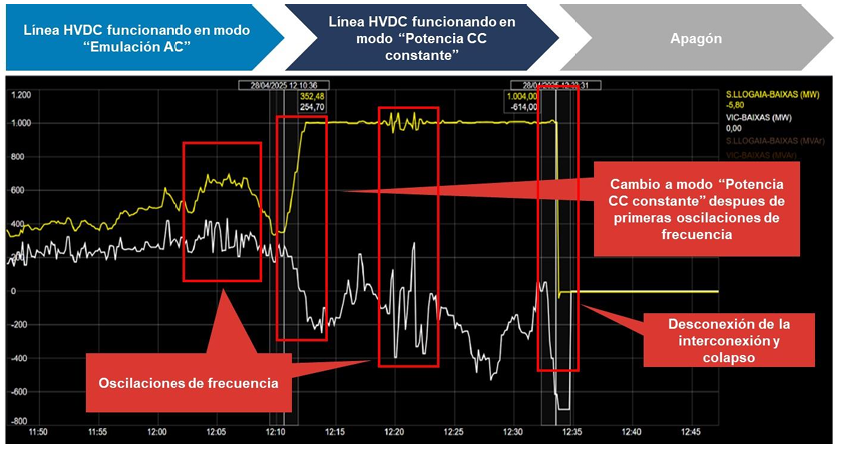
\includegraphics[width=0.85\textwidth]{figuras/hvdc_control_transition.png}
    \caption[Cambio del modo de control en el enlace HVDC INELFE-1 España-Francia.]{%
    Cambio del modo de control en el enlace HVDC INELFE-1 España-Francia.
    Fuente: Informe IIT-ICAI / AELEC}
    \label{fig:hvdc_control}
\end{figure}

\subsection{Frontera sur (Marruecos)}

El sistema peninsular se conecta con el norte de África mediante cables
submarinos de corriente alterna (AC) a través del Estrecho de Gibraltar, con una
capacidad técnica de 900~MW. Momentos antes del colapso, España importaba
314~MW desde Marruecos. A las 12:33:20~CEST, los relés de subfrecuencia del
operador marroquí dispararon al alcanzarse el umbral de 49,5~Hz,
desconectando el enlace para proteger su red ante una propagación de las inestabilidades del sistema español \cite{ree2025}.

Esta desconexión, aunque protectora para Marruecos, tuvo consecuencias
relevantes en la fase de reposición: la inyección de tensión importada desde
el sur horas más tarde proporcionó la referencia necesaria para iniciar las
estrategias de arranque autónomo (\textit{Black Start}) de los ciclos
combinados de Andalucía \cite{gobierno2025}.

\clearpage

\section{El Sistema de Alerta Europeo (EAS): estado de la red según los estándares
de ENTSO-E antes del incidente}
\label{sec:eas_entsoe}

\subsection{Definición y función del sistema de vigilancia de ENTSO-E}

La coordinación de la seguridad en el área síncrona de Europa continental se
articula a través del sistema de vigilancia de ENTSO-E (\textit{ENTSO-E
Awareness System}, EAS). Esta plataforma constituye el pilar de la
monitorización paneuropea: proporciona a los Gestores de Redes de Transporte
(TSOs) y a los Centros de Coordinación Regional (RCCs) una visión en tiempo
real del estado operativo de la red síncrona, permitiendo el intercambio
instantáneo de parámetros críticos y la toma de decisiones conjuntas ante
situaciones de estrés \cite{entsoe2025}.

\subsection{Clasificación de los Estados Operativos (SO GL)}

Para estandarizar la evaluación de la seguridad, la normativa europea
(\textit{System Operation Guidelines}, SO GL) establece cinco niveles progresivos
de severidad \cite{entsoe2025}:

\begin{itemize}
    \item \textbf{Normal (\textit{Normal state}):} el sistema opera dentro de los
    límites de seguridad, cumpliendo el Criterio $N-1$.

    \item \textbf{Alerta (\textit{Alert state}):} degradación de los márgenes de
    seguridad ---reservas, tensión o frecuencia--- que exige acciones preventivas.

    \item \textbf{Emergencia (\textit{Emergency state}):} violación de límites de
    seguridad, pérdida de sincronismo o activación de deslastre de cargas (UFLS).

    \item \textbf{Apagón (\textit{Blackout state}):} pérdida total de tensión en
    una parte significativa de la zona de control.

    \item \textbf{Restauración (\textit{Restoration state}):} implementación de
    estrategias de \textit{Black Start} y reposición topológica de la red.
\end{itemize}

\subsection{Estado previo al incidente: la ``falsa normalidad'' de la Fase~0}

El análisis de los registros del EAS revela una disonancia entre la dinámica
de la red ibérica y su representación en la plataforma europea. Durante la
mañana del 28 de abril, el sistema sufrió, al menos, dos oscilaciones
significativas: una oscilación forzada de 0,6~Hz a las 12:03~CEST y un modo
inter-área de 0,2~Hz a las 12:19~CEST. Ambas obligaron a Red Eléctrica
(REE) a ejecutar maniobras de mallado cuyo efecto sobre el perfil de
tensiones es objeto de interpretación divergente entre los informes: el
informe pericial del IIT-ICAI sostiene que dichas maniobras pudieron
contribuir a saturar la capacidad de absorción de potencia reactiva de la
red, mientras que la posición de REE ---desarrollada en el
capítulo~\ref{cap:analisis_informes}
(p.~\pageref{cap:analisis_informes})--- es que las maniobras se ajustaron a
los procedimientos establecidos y no constituyeron causa raíz del incidente
posterior \cite{entsoe2025}.

A pesar de la gravedad de estos fenómenos, ni el operador español (REE) ni el
portugués (REN) declararon el estado de Alerta en el EAS. A las 12:32:00~CEST,
el estado oficial declarado para la península ibérica seguía siendo ``Normal''. Los
registros confirman que el sistema transitó abruptamente de ``Normal'' a
``Blackout'' (criterio OB3) a las 12:33:29~CEST, sin haber pasado preventivamente
por ninguna de las fases intermedias \cite{entsoe2025}.

\begin{figure}[H]
    \centering
    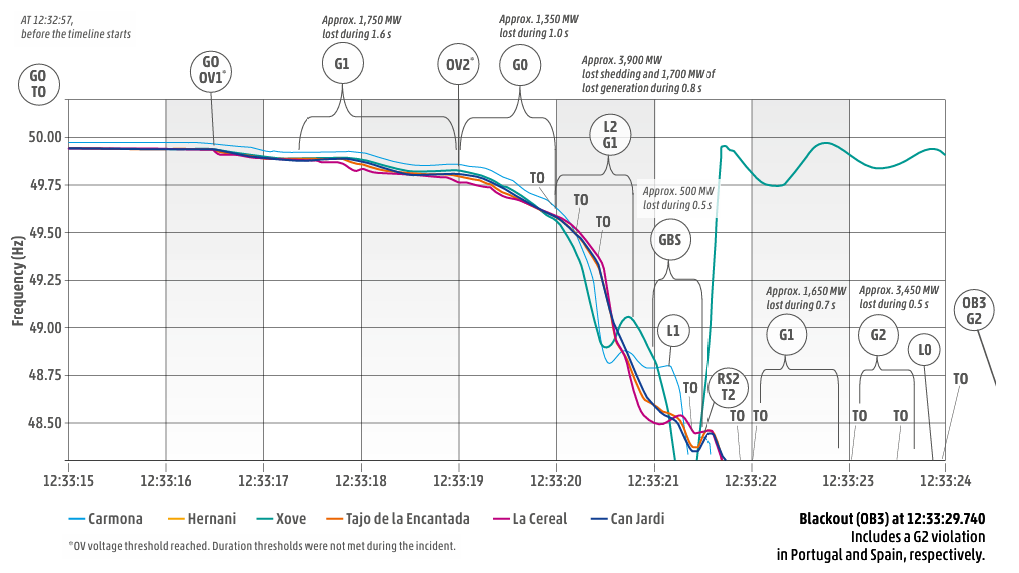
\includegraphics[width=0.85\textwidth]{figuras/ics_violations_iberia.png}
    \caption[Clasificación de las violaciones de seguridad (Criterios ICS) en la
    península ibérica.]{%
    Clasificación de las violaciones de seguridad (Criterios ICS) en la
    península ibérica. Los registros oficiales constatan que el sistema fue
    catalogado en estado de Apagón (criterio OB3) a posteriori, sin una
    declaración previa de Alerta.
    Fuente: Informe Factual ENTSO-E}
    \label{fig:ics_violations}
\end{figure}

\subsection{Visibilidad transfronteriza y la ``ceguera'' del sistema europeo}

La ausencia de escalada en los estados de seguridad generó una situación de
visibilidad limitada hacia los operadores vecinos. Los monitores del área
síncrona (Swissgrid) y el Centro de Coordinación Regional (Coreso) percibían
una robustez técnica estándar en el bloque ibérico. El operador francés (RTE)
no recibía señales que indicasen una vulnerabilidad dinámica al sur de los
Pirineos: al permanecer el EAS en estado ``Normal'', no se activaron protocolos
de cooperación transfronteriza ni se preparó la red francesa para el
transitorio que afectó a la frontera a las 12:33:21~CEST \cite{entsoe2025}.

El episodio puso de manifiesto que el EAS actuó no como una herramienta de
alerta temprana (\textit{early warning}), sino como un notificador
\textit{post mortem} del colapso. Esta limitación estructural ---la capacidad
limitada del sistema europeo de monitorización para capturar la dinámica
rápida de tensión en redes de baja inercia--- constituye una de las lecciones
regulatorias centrales del incidente \cite{mitceepr2025}.

\begin{figure}[H]
    \centering
    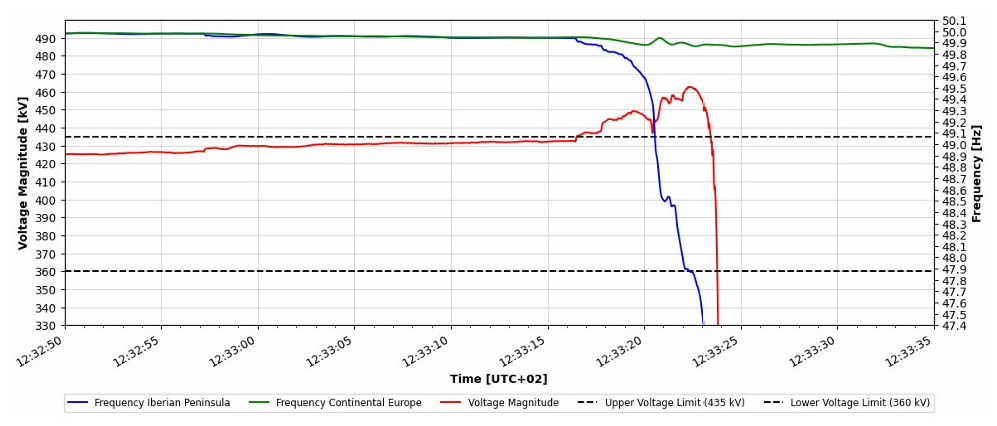
\includegraphics[width=0.85\textwidth]{figuras/frequency_voltage_carmona.png}
    \caption[Evolución de la frecuencia y la tensión en la subestación de Carmona (Sevilla).]{%
    Evolución de la frecuencia y la tensión en los segundos críticos del
    incidente (Subestación de Carmona, 400~kV). Fuente: Informe Factual
    ENTSO-E / REE}
    \label{fig:carmona_oscilogram}
\end{figure}